%%%% PROCESAR con PdfLaTeX !!!!!


\documentclass[12pt]{book}
\usepackage{geometry}\geometry{top=2cm,bottom=2cm,left=3cm,right=3cm}
\usepackage{amssymb}
\usepackage{amsmath}
\usepackage{graphicx}
\usepackage{txfonts}
\usepackage[latin1]{inputenc}
\usepackage[usenames]{color}



\begin{document}
\thispagestyle{empty}

\begin {center}


\includegraphics[scale=.4]{Logo-fiuba_big.png}

\medskip
UNIVERSIDAD DE BUENOS AIRES

Facultad de Ingenier\'ia

Departamento de Economia, Organizaci\'on y legal


\vspace{3cm}


\textbf{\large 7114 Modelos y Optimizaci\'on 1}
\\
\textbf{\large Pr\'actica 1}
\vspace{2cm}


Este es un modesto aporte para los alumnos de la f\'acultad de ingenier\'ia  de la UBA de las carreras de licenciatura en an\'alsis de sistemas e ingenier\'ia inform\'atica.
De ninguna man\'era pretende ser una gu\'ia de estudio, ni remplaza las clases presenciales, el material oficial de la catedra esta disponible en el web site de la m\'ateria.
\\
wwww.ModelosUno.com.ar

\end {center}


\vspace{2.5cm}

\noindent Autor:	Isaac Edgar Camacho Ocampo
 
\noindent Carrera:	Licenciatura en An\'alisis de sistemas

\vspace{1cm}

\vspace{1cm}

\noindent Buenos Aires, 2019

\newpage

%EJERCICIO 1
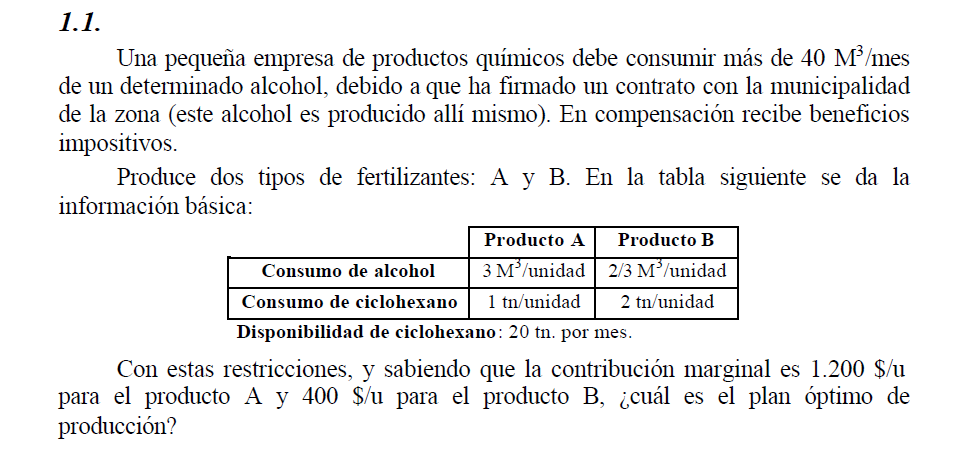
\includegraphics[scale=.6]{ej1.png}
\linebreak
\linebreak
\\
\begin{large}
Resoluci\'on
\end{large}
\\
\\
\textbf{Objetivo: }determinar la cantidad de productos A y B a fabricar en un mas para maximizar las ganancias.
\\
\\
\textbf{Hip\'otesis: }
\begin{enumerate}
\item no existen m\'ermas en el proceso de producci\'on.
\item todo lo que se produce se vende, es decir que la demanda no es limitante.
\item no existe acumulaci\'on de stock.
\end{enumerate}
\textbf{Variables :}
\begin{itemize}
\item $P_a [\frac{unidades}{mes}]$: cantidad fabricada de producto tipo A
\item $P_b [\frac{unidades}{mes}]$: cantidad fabricada de producto tipo B 
\end{itemize}
\textbf{Inecuaciones: }
\begin{itemize}
\item $3 [\frac{m^3}{unidad}]  P_a[\frac{unidades}{mes}] + 2/3 [\frac{m^3}{unidad}]  P_b [\frac{unidades}{mes}] \geq 40 [\frac{m^3}{mes}]  $ \, \textit{(Consumo de alcohol)}

\item $1 [\frac{ton}{unidad}]  P_a[\frac{unidades}{mes}] + 2 [\frac{ton}{unidad}]  P_b [\frac{unidades}{mes}] \leq 20 [\frac{ton}{mes}]  $ \, \textit{ (Consumo de ciclohexano}
\end{itemize}
\pagebreak
\textbf{Funcional: }El funcional hace que las variables $P_a$ y $P_b$ tomen valores lo m\'as grandes posibles teniendo en cuenta que el ciclohexano tiene un l\'imite en su disponibilidad y por otro lado el alcohol tiene un consumo m\'inino.
\begin{itemize}
\item $Z_{max} \Rightarrow 1200 [\frac{\$}{unidad}]  P_a[\frac{unidades}{mes}] + 400 [\frac{\$}{unidad}]  P_b [\frac{unidades}{mes}] $
\end{itemize}

\begin{center}
\textbf{Resoluci\'on gr\'afica}
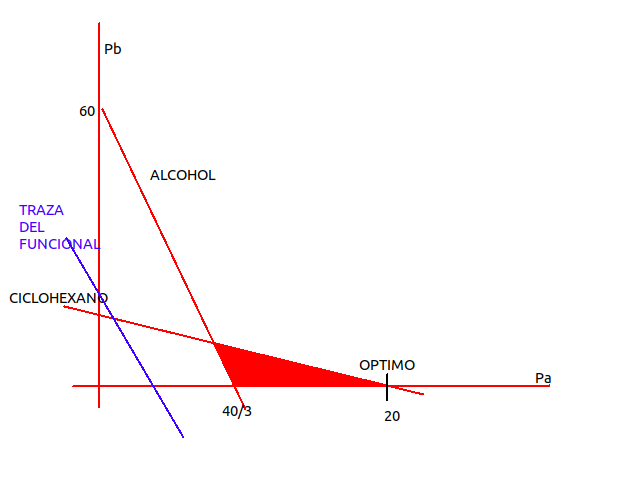
\includegraphics[scale=.5]{ej1_graf.png}
\end{center}


\end{document}

